\documentclass[nobib]{tufte-handout}
\usepackage{etex} \reserveinserts{36}
\usepackage{graphicx}
\usepackage{morefloats}
\setkeys{Gin}{width=\linewidth,totalheight=\textheight,keepaspectratio}
\graphicspath{{figures/}}
\usepackage[numbers,square,sort&compress]{natbib}

% The units package provides nice, non-stacked fractions and better spacing
% for units.
% \usepackage{units}

% The fancyvrb package lets us customize the formatting of verbatim
% environments.  We use a slightly smaller font.
\usepackage{fancyvrb}
\fvset{fontsize=\normalsize}

% Small sections of multiple columns
% \usepackage{multicol}

% Brief personal statement addressing current research, professional contributions, and future goals



\hypersetup{colorlinks}

\newcommand{\minisec}[1]{\vspace{3pt} \noindent \emph{#1}\ }

\title{Research statement}
\author{\href{http://matsen.fredhutch.org/}{Frederick A Matsen IV}\\Fred Hutchinson Cancer Research Center}


\begin{document}

\maketitle

\begin{abstract}
\noindent
As large biological data sets become easily available, methodological advances in computational biology can greatly improve our understanding of hidden processes.
I am committed to building rigorous computational methods to solve important problems in biology and to making those tools accessible to biologists.
Guided by collaborative work on hard problems in biomedicine, I develop sequence analysis methods that integrate relevant biological details, deliver meaningful uncertainty estimates, and scale to large data sets.

In the past five years my group initiated a transition from performing classical inference under classical probabilistic models to our next phase: making inferences under models without easily computed likelihoods, as well as developing next-generation inferential tools that move beyond the classical algorithmic toolbox.
In the next five years, we will develop
\begin{enumerate}
\item variational Bayesian phylogenetic inference into an efficient, feature-rich, and mature inferential method
\item neural-network-based methods to study B cell somatic hypermutation and T cell receptor sequence diversity.
\end{enumerate}
\end{abstract}

\begin{marginfigure}[1.8in]%
  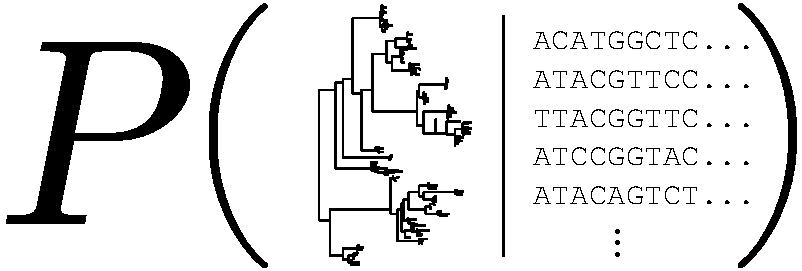
\includegraphics[width=1.95in]{bayesian_phylo}
  \caption{\
The objective of Bayesian phylogenetic inference is to infer a posterior distribution on phylogenetic trees, giving the probability that each tree is correct given sequence data.
    }
  \label{FIGbayesPhylo}
\end{marginfigure}%


\vspace{0.3cm}
\section{Next-generation methods for Bayesian phylogenetic inference}
\vspace{-0.3cm}
The goal of Bayesian phylogenetic inference is to infer a posterior distribution on evolutionary trees given some sequence data (Fig.~\ref{FIGbayesPhylo}).
Because evolutionary signal is sparse for our domain of interest (pathogens and B cell receptors), and phylogenetic models are parameter-rich, we observe considerable uncertainty in inferences.
Bayesian methods directly report that uncertainty, and make it possible to pass the uncertainty on to another phase of analysis.
% For example, we have found in collaborative work with the Overbaugh lab \cite{Simonich2019-nn} that B cell receptor phylogenetic trees show substantial uncertainty in their structure and ancestral sequences.
We want to make such probabilistic analysis much more efficient so that researchers can be more confident in their inferences.

\newthought{Current Bayesian phylogenetic methods do not scale} to modern data sets.
These methods are based on the classical Markov chain Monte-Carlo (MCMC) algorithm, which performs random tree modifications (Fig.~\ref{FIGsprdef}) whereby modifications that result in better (higher likelihood) trees are favored over jumps to worse trees.
However, most of these random modifications will result in a significantly worse tree, and thus are not accepted by the algorithm.
Such low acceptance rates make MCMC inapplicable to large data sets.

\begin{marginfigure}[-1.9in]%
  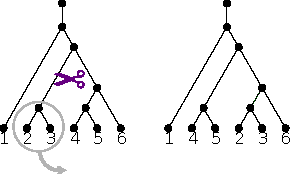
\includegraphics[width=1.95in]{spr-definition}
  \caption{\
    A phylogenetic tree and the result of applying a subtree-prune-regraft (SPR) modification to it.
    In this modification, a subtree is cut off the larger tree, then reattached using a new edge (dotted line of right hand tree).
    }
  \label{FIGsprdef}
\end{marginfigure}%

In the past five years we have been obsessed with finding a scalable alternative to MCMC, developing phylogenetic methods based on
sequential Monte Carlo \cite{Dinh2017-sh,Fourment2017-an,Claywell2018-zg},
Hamiltonian Monte Carlo \cite{Dinh2017-oj},
systematic search \cite{Whidden2018-db} with efficient marginal likelihood estimation \cite{Fourment2018-xx},
and variational inference \cite{Zhang2018-lw,Zhang2018-mm}.
Of these, variational inference is by far the most promising.

Variational inference fits a so-called variational approximation to a posterior distribution (Fig.~\ref{FIGvariationalGradient}) rather than sampling from it.
Accurate variational inference methods depend on a variational approximation that can closely match the true posterior distribution.
% It is not immediately obvious how to define a good variational approximation on the set of phylogenetic trees.
%, an intricate mixture of discrete and continuous components.

\begin{marginfigure}[0.in]%
  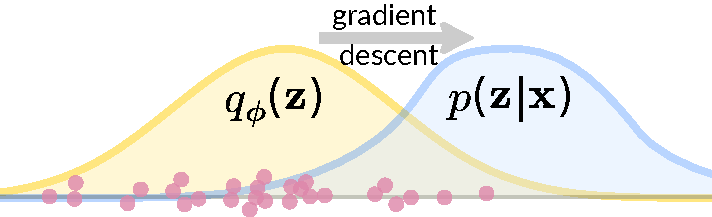
\includegraphics[width=1.95in]{variational-gradient}
  \caption{\
    Variational inference fits an approximating distribution $q_\phi$ to the posterior $p$ by modifying parameters $\phi$.
    Pink circles schematize samples from the current approximate posterior; having these samples in hand enables efficient gradient descent steps to fit $q_\phi$.
    }
  \label{FIGvariationalGradient}
\end{marginfigure}%

Our variational inference method is formulated in terms of conditional probabilities of splitting events on trees (Fig.~\ref{FIGcsd}).
We have shown that such a parameterization is sufficiently rich to capture the structure of real phylogenetic posterior distributions \cite{Zhang2018-mm}.
In fact, we showed that fitting such a distribution to an MCMC sample of phylogenetic trees results in a better approximation to the posterior than simply using the MCMC samples, showing that the ``information sharing'' inherent in our parameterization smooths out MCMC stochasticity.

\begin{marginfigure}[0.7in]%
  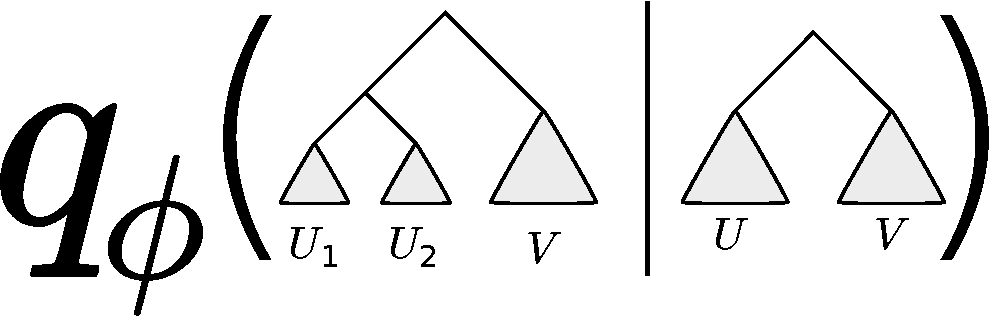
\includegraphics[width=1.95in]{csd}
  \caption{\
    A tree topology can be broken down into a collection of conditional statements about splitting of subtrees.
    Our variational parameterization on tree topologies approximates a posterior on tree topologies as a product of conditional probabilities about these splitting steps.
    }
  \label{FIGcsd}
\end{marginfigure}%

We then developed full variational inference by combining this variational parameterization on phylogenetic tree topologies with a parameterization on tree branch lengths \cite{Zhang2018-lw}.
We showed that our variational methods quickly approximate the posterior (Fig.~\ref{FIGvbpiPerformance}).

\begin{marginfigure}[0.7in]%
  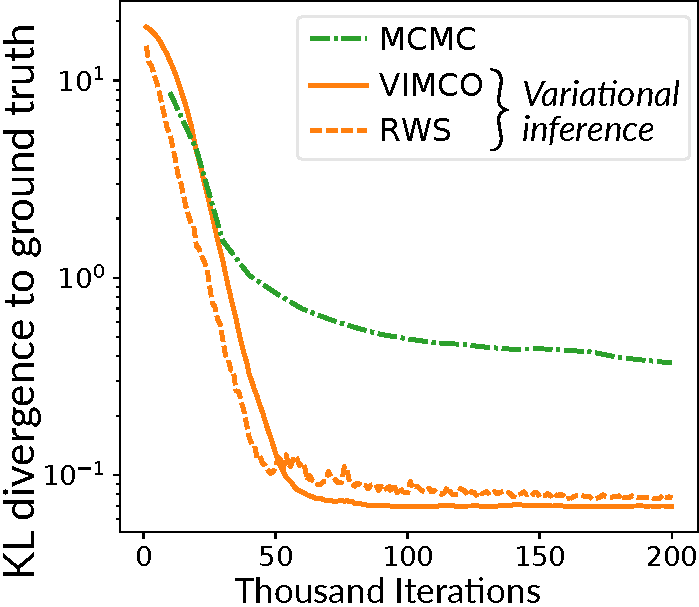
\includegraphics[width=1.95in]{vbpi-performance}
  \caption{\
    The performance of direct variational Bayes phylogenetic inference on benchmark data set DS1 (lower is better).
    Figure simplified from \cite{Zhang2018-lw}.
    }
  \label{FIGvbpiPerformance}
\end{marginfigure}%

\paragraph{Future plans}
We are moving quickly to build variational Bayesian inference into a complete inferential framework.
This includes developing \href{https://github.com/phylovi/libsbn/}{libsbn}, a Python-interface C++ library to provide efficient implementations of the algorithmic core of variational Bayes phylogenetic inference and thus enable researchers to develop complex phylogenetic models using Python-based modeling platforms such as \href{https://www.tensorflow.org/}{Tensorflow} and \href{https://pytorch.org/}{PyTorch}.
We are also developing methods to allow divide-and-conquer Bayesian phylogenetic inference, which we believe is an essential component of scaling phylogenetic inference to large data sets.
Farther down the road, we also believe that variational methods can enable whole-sequence-based phylogenetic inference methods, which will allow us to avoid the ubiquitous and problematic independence-across-sites assumption.


\vspace{0.3cm}
\section{Deep learning for immune repertoires}
\vspace{-0.3cm}

The adaptive immune system is composed of B and T cells, each of which has a highly adaptable and variable receptor to bind a very diverse and ever-changing landscape of antigens.
B cell receptors (BCRs), called antibodies in their secreted form, bind directly to antigens (Fig.~\ref{FIGbcrTcr}).
T cell receptors (TCRs) do not have a secreted form, and bind cleaved antigen-derived peptides that are presented by Major Histocompatibility Complex (MHC).
BCRs and TCRs are incredibly diverse, being generated by a within-individual random process that begins with V(D)J recombination.
One can apply high-throughput sequencing to the DNA encoding these BCRs and/or TCRs to obtain millions of unique adaptive immune receptor sequences from a single blood draw, giving what is called an immune repertoire.

\begin{marginfigure}[-0.4in]%
\begin{centering}
  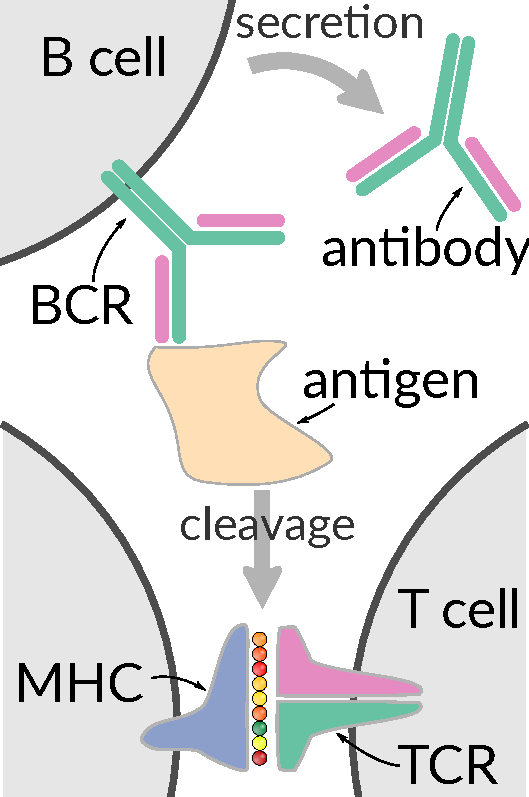
\includegraphics[width=1.5in]{bcr-tcr}
\end{centering}
  \caption{\
    B cell receptors (BCRs) and T cell receptors (TCRs).
    }
  \label{FIGbcrTcr}
\end{marginfigure}%

During our first five years of working on immune repertoires, we used existing statistical frameworks to learn about the generative process of antibodies and T cell receptors \cite{McCoy2015-qi, Ralph2016-kr, Ralph2016-yl, Ralph2017-ih, DeWitt2018-el, Dhar2018-ne, Zhang2018-gn, Davidsen2018-gn, DeWitt2018-ar, Simonich2019-nn, Feng2019-sj, Dhar2019-qg}.
However, as we described in an invited review \cite{Olson2018-lw}, some key aspects of immunology are simply out of reach using classical methods.
For example, although simple probabilistic models such as hidden Markov models (HMMs) work very well to characterize the first rearrangement step, tolerance checkpoints and expansion involve functional binding properties that cannot be represented by such simple probabilistic models.
We are thus now using non-classical methods:
first, we use deep neural networks for receptor analysis, and second, we develop and fit mechanistic probabilistic models for the intricate process of somatic hypermutation.

\begin{marginfigure}[0.1in]%
\begin{centering}
    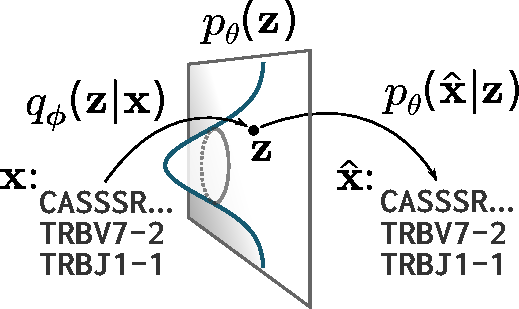
\includegraphics[width=1.9in]{figures/vae.pdf}
\end{centering}
  \caption{\
    Our variational autoencoder (VAE) embeds TCR protein sequences $\mathbf{x}$ into an $n$-dimensional latent space, using a probabilistic encoder $q_\phi$ and decoder $p_\theta$ that are both parametrized by deep neural networks.
The VAE objective is to encode and decode objects with high fidelity while ensuring the encoder distribution is close to a prior $p_\theta(\mathbf{z})$ on that latent space.
    }
  \label{FIGvae}
\end{marginfigure}%

% Although simple probabilistic models such as hidden Markov models (HMMs) work very well to characterize the first rearrangement step, tolerance checkpoints and expansion involve functional binding properties that cannot be represented by such simple probabilistic models.
% Indeed, binding is a property of the entire receptor, introducing long-range dependencies that cannot be broken down into simple conditional probabilities.
% To do better, one needs a more flexible model and lots of data.


\subsection*{Deep generative models}
Our group is advancing beyond the state of the art by developing generative models built from deep neural networks.
% These models are similar to classical models, such as HMMs, in that they can be fit to an observed distribution of sequences and can generate additional sequences.
% However, neural networks are much more flexible, and thus can represent more complex distributions.
Our first step is to use variational autoencoders (VAEs) \cite{Kingma2014-mo} to learn complex sequence distributions.
VAEs use an encoder network, a decoder network, and a distribution on an embedding space, to give a generative model (Fig.~\ref{FIGvae}).
We train the VAE using collections of sequence data and then can use it to assess probability of given sequences \cite{Davidsen2019-uw}.
For example, we perform more accurate frequency estimation on the data set of \cite{Emerson2017-co} compared to an existing model (Fig.~\ref{FIGfrequency}).

\begin{marginfigure}[0.2in]%
\begin{centering}
    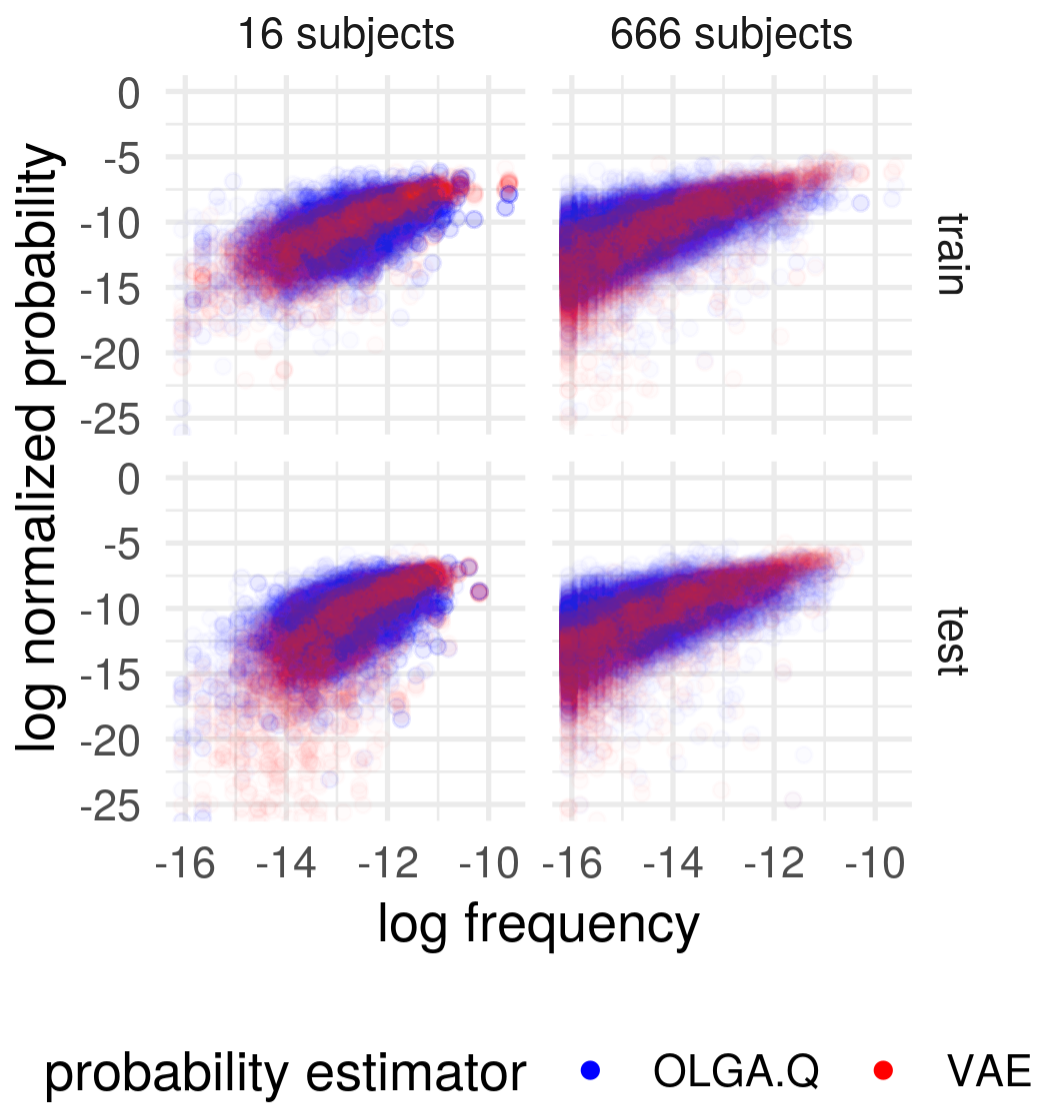
\includegraphics[width=\textwidth]{log_normed_Ppost_vs_log_normed_Pvae.png}
\end{centering}
  \caption{\
    Our VAE provides more accurate frequency estimates compared to a state-of-the-art recombination model with a simple selection model.
    }
  \label{FIGfrequency}
\end{marginfigure}%

\subsection*{Somatic hypermutation}

Somatic hypermutation (SHM) is the driver of affinity maturation: the within-host process by which antibodies gain high affinity.
Thus to understand prospects for eliciting specific antibodies through vaccination we must estimate mutation probability accurately.
% Accurate estimation of SHM mutation probability is important for understanding which antibodies are accessible from a certain na\"ive progenitor cell.
% For example, it has been shown that specific low-probability mutations are important for broadly-neutralizing HIV antibody maturation \cite{Bonsignori2017-nj,Hwang2017-tt,Wiehe2018-of}.
% Thus to understand prospects for eliciting such antibodies through vaccination, and how to design vaccine inserts rationally \cite{Jardine2013-yt}, we must estimate mutation probability accurately.

The current statistical approach works to understand the influence of local sequence context, namely the surrounding DNA bases, on mutation probability \cite{Rogozin1992-xv,Yaari2013-dg,Cui2016-wz}.
We have ourselves extended this work with a penalized  proportional hazards model \cite{Feng2019-sj} that takes the influence of earlier mutations on later mutations, and only allows parameters into the model when they improve model fit.
However, the accuracy of these local models is inherently limited by the width of the local sequence context that they examine (Fig.~\ref{FIGshm}).

We are now moving beyond these limitations by directly fitting mechanistic models of SHM, which are parameterized in terms that have direct biological significance, such as transcription bubble size and probabilities of various repair pathways.
These complex models do not admit a likelihood so cannot be fit with classical means.
Therefore we are developing neural network methods to perform parameter inference, along the lines of \cite{Jiang2017-xs,Chan2018-qq}.


\begin{marginfigure}[0.in]%
\begin{centering}
    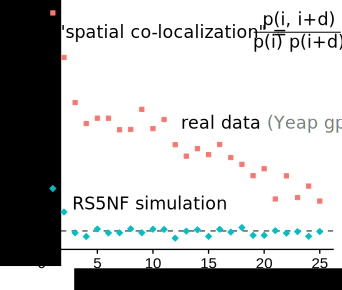
\includegraphics[width=\textwidth]{spatial-co-localization}
\end{centering}
  \caption{\
   Current models such as RS5NF \cite{Cui2016-wz} do not capture the clustering of mutations seen in real data \cite{Yeap2015-nl} as measured by the ``spatial co-localization'' \cite{Marcou2018-sm} quantifying non-independence of mutations separated by a distance $d$.
    }
  \label{FIGshm}
\end{marginfigure}%

\paragraph{Future plans}
Our immediate future plans are to continue developing generative models of immune repertoires, including a na\"ive B cell probability estimator that can be used to rank prospective antibodies in terms of their elicitation potential.
We will also investigate the degree to which such models can aid in T cell binding prediction.
For the SHM work, we now have funding to investigate SHM in a model laboratory system with Hedda Wardemann's group.


\section{Collaborations and broader impacts}

Although I have focused on our future directions that are more methodologically ambitious, we will continue to develop methods based on classical foundations that are of more immediate utility.
For example, we have just finished a Bayesian phylogenetic hidden Markov model for B cell receptor sequences \cite{Dhar2019-qg}, which provides B cell naive sequence estimates with corresponding estimates of certainty for the first time.
These sequences are being built into antibodies and tested by the Overbaugh lab for their research.

I will also continue to move forward my community-building and educational efforts.
At Fred Hutch, I will continue to advise \href{http://fredhutch.io/}{fredhutch.io} educational initiative that I started in 2014.
I will also continue to organize and host \href{http://phyloseminar.org/}{phyloseminar.org}, an online seminar series on phylogenetics which has had 89 talks and over 56,800 views, as well as the \href{http://b-t.cr/}{B-T.CR} forum on BCR and TCR sequence analysis.



\newpage
\bibliography{main}
\bibliographystyle{abbrvunsrtnat}


\newpage

\section{Diversity statement}

I am very glad to hear that Fred Hutch has decided to make diversity and inclusion part of the promotion process.
However, my performance in this realm has been mixed.

On one hand I have done a good job of bringing a diverse group of interns for summer projects in my group.
We have had 8 interns since 2014, 5 of which were women, and 6 of which were not Caucasian.
All of these students had a significant experience writing scientific software, and many are still in touch and doing great things.
I also view my work on \href{http://phyloseminar.org/}{phyloseminar.org} as having an inclusiveness component, as these seminars reach a truly global audience.

However, my track record of recruiting women and under-represented minorities into the group has been poor.
I have only had one woman PhD student and one woman postdoc.
Both of these individuals have been very successful.

I have discussed my shortcomings in recruiting with Julie Overbaugh and have developed a new plan of finding candidates well before their graduation and cultivating their interest in our research program.
I would welcome any other advice or assistance.



\end{document}
